\documentclass[conf]{new-aiaa}
%\documentclass[journal]{new-aiaa} for journal papers
\usepackage[utf8]{inputenc}

\usepackage{graphicx}
\usepackage{amsmath}
\usepackage[version=4]{mhchem}
\usepackage{listings}
\usepackage{color}
\usepackage{siunitx}
\usepackage{longtable,tabularx}
\usepackage{subcaption}
\usepackage{cleveref}
\usepackage{appendix}
\setlength\LTleft{0pt}

\title{AE602 - Compressible Flow Assignment - 03}

\author{Ramkumar S. \footnote{SC22M007, M.Tech., Aerospace AFM }}
\affil{SC22M007, M.Tech. Aerospace - Aerodynamics and Flight Mechanics}


\definecolor{mygreen}{rgb}{0,0.6,0}
\definecolor{mygray}{rgb}{0.5,0.5,0.5}
\definecolor{mymauve}{rgb}{0.58,0,0.82}

\lstset{
  backgroundcolor=\color{white},   % choose the background color; you must add \usepackage{color} or \usepackage{xcolor}; should come as last argument
  basicstyle=\footnotesize,        % the size of the fonts that are used for the code
  breakatwhitespace=false,         % sets if automatic breaks should only happen at whitespace
  breaklines=true,                 % sets automatic line breaking
  captionpos=b,                    % sets the caption-position to bottom
  commentstyle=\color{mygreen},    % comment style
  deletekeywords={...},            % if you want to delete keywords from the given language
  escapeinside={\%*}{*)},          % if you want to add LaTeX within your code
  extendedchars=true,              % lets you use non-ASCII characters; for 8-bits encodings only, does not work with UTF-8
  firstnumber=0001,                % start line enumeration with line 1000
  frame=single,                    % adds a frame around the code
  keepspaces=true,                 % keeps spaces in text, useful for keeping indentation of code (possibly needs columns=flexible)
  keywordstyle=\color{blue},       % keyword style
  language=Octave,                 % the language of the code
  morekeywords={*,...},            % if you want to add more keywords to the set
  numbers=left,                    % where to put the line-numbers; possible values are (none, left, right)
  numbersep=5pt,                   % how far the line-numbers are from the code
  numberstyle=\tiny\color{mygray}, % the style that is used for the line-numbers
  rulecolor=\color{black},         % if not set, the frame-color may be changed on line-breaks within not-black text (e.g. comments (green here))
  showspaces=false,                % show spaces everywhere adding particular underscores; it overrides 'showstringspaces'
  showstringspaces=false,          % underline spaces within strings only
  showtabs=false,                  % show tabs within strings adding particular underscores
  stepnumber=2,                    % the step between two line-numbers. If it's 1, each line will be numbered
  stringstyle=\color{mymauve},     % string literal style
  tabsize=2,                       % sets default tabsize to 2 spaces
  % title=\lstname                 % show the filename of files included with \lstinputlisting; also try caption instead of title
}

\begin{document}

\maketitle

\begin{abstract}
    The present work is about solving the given supersonic flow over an
    expansion corner problem using the Method of Characteristics. The inlet
    Mach number is specified to be 3.0 and the flow deflection angle is
    given to be $\theta = 15^{\circ}$, the duct height is 30 cm. and the
    length of the expansion section is taken to be 120 cm.
\end{abstract}


\section{Question}

\begin{figure*}[!h]
    \center
    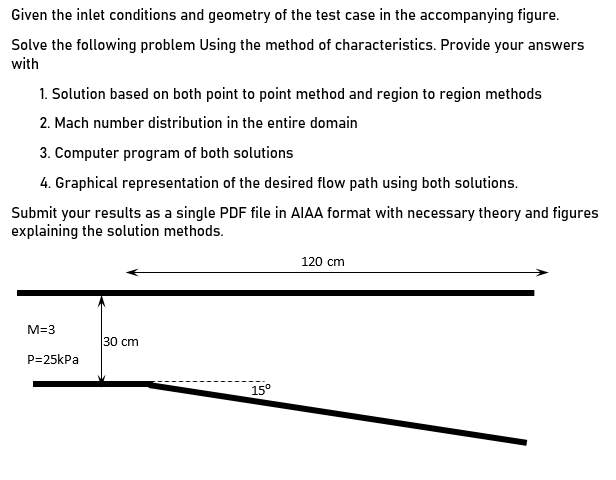
\includegraphics[scale=0.5]{results/question.png}
\end{figure*}

\textbf{SOLUTION:}\\

\par Given data
\begin{align*}
    M_1 &= 3.0 \\
    h &= 0.3 \ m \\
    L &= 1.2 \ m \\
    P_1 &= 25 \ kPa
\end{align*}

\par The solution algorithm followed for this problem is given below.\\

\par The number of characteristic nodes N, in the inlet plane is first chosen. The
value chosen for this problem is 100. An example layout of Characteristic lines
with N = 6, in the expansion flow domain of deflection angle $2^{\circ}$ is given in
\Cref{domain_layout}.But, the actual problem with $15^{\circ}$ deflection angle
requies N = 100 in order to accurately capture the expansion flow field. \\

\begin{figure}
   \center
    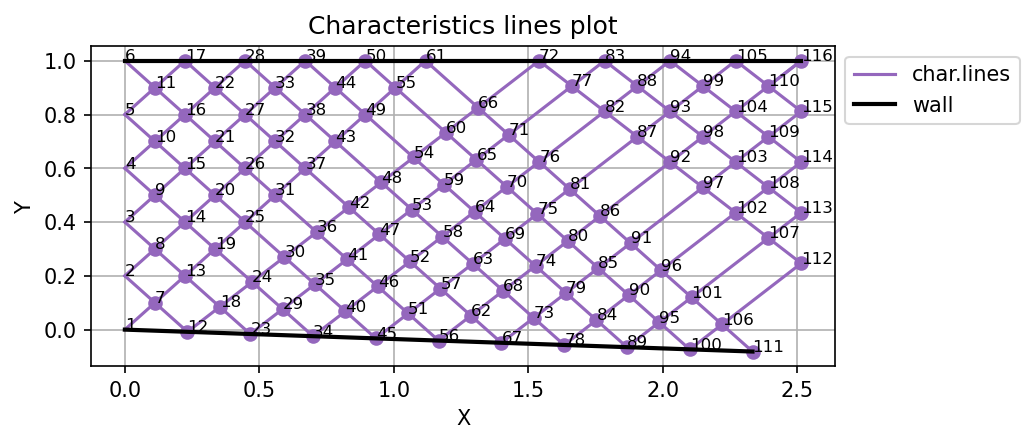
\includegraphics[scale=0.9]{results/expansion_corner_trial/char_map.png}
    \caption{Coarse characteristic points layout on the $2^{\circ}$ expansion corner}
    \label{domain_layout}
\end{figure}

\par Then the total number of characteristic nodes that will appear after all
interactions is computed using the equation below. Here, $n_{wall}$ is the number
of wall bounces requried as it is the one that controls the length of the
computation domain in this case. \\
\begin{align*}
    N_{total} = n_{wall} (2 N - 1) + N
\end{align*}

\par After this, a list of numbers indicating the characteristic points were
generated linearly similar to the one shown in \Cref{domain_layout} and the
points on both top and bottom wall is identified using the below equations
and were grouped for ease of computation.
\begin{align*}
    bottom\ wall: n_b = n_{b,prev} + (2N -1) \\
    top\ wall: n_b = n_{b,prev} + (N -1) \\
\end{align*}

\par Then a table, with the list of dependence upstream characteristic points,
to each internal and boundary char.point is made, which will be used during
computations. The inlet condition is defined such that, the expansion function
values $\nu(M)$ at all inlet char.points is computed for the following specified
condition. And the values of $K_1$ and $K_2$ were computed using the relations
given.
\begin{align*}
    M_{inlet} &= 3.0  \\
    \theta_{inlet} &= 0.0 \\
    K_1 &= \nu + \theta \\
    K_2 &= \nu - \theta
\end{align*}

\par Then the computation is begun for internal points, where the values of
$\nu$ and $\theta$ were computed by taking the intersected $K_1$ and $K_2$
upstream values as shown below.
\begin{align*}
    \nu &= \frac{K_1 + K_2}{2} \\
    \theta &= \frac{K_1 - K_2}{2}
\end{align*}

\par At the wall points, only one upstream characteristics meet, but the
wall angle $\theta_{wall}$ is known, hence using the upstream characteristic
and wall angle values, the expansion function is computed as shown in the
example below.
\begin{align*}
    bottom\ wall: \nu &= K_1 - \theta \\
    top\ wall: \nu &= K_2 + \theta
\end{align*}

\par Then, the Mach numbers at each characteristic point were computed using
Prandtl-Meyer expansion function relation given below.
\begin{align*}
    \nu(M) = \sqrt{\frac{\gamma+1}{\gamma-1}}tan^{-1}\sqrt{\frac{\gamma-1}{\gamma+1}\left(M^2-1\right)} - tan^{-1}\sqrt{M^2-1}
\end{align*}

\par For computing the location of downstream char.point, the following equations
that determine the slope of line (with the assumption that the char. curves are
straight lines in short length) and the location of the point as shown in the
\Cref{slope_image}.
\begin{figure}
    \center
    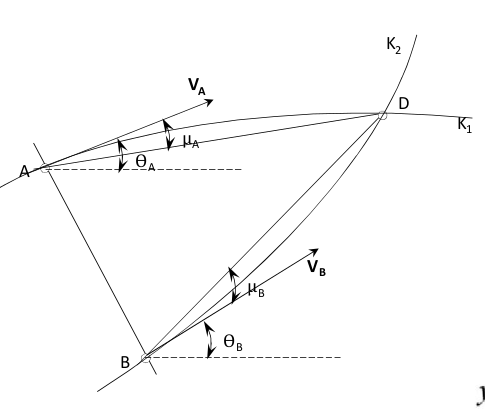
\includegraphics[scale=0.5]{results/slopeImage.png}
    \caption{reference image for the char. point position calculations}
    \label{slope_image}
\end{figure}


\begin{align*}
    \left(\frac{dy}{dx}\right)_A &= tan(\theta-\mu)_A \\
    \left(\frac{dy}{dx}\right)_B &= tan(\theta+\mu)_B \\
    S_1 &= \frac{tan(\theta-\mu)_A + tan(\theta-\mu)_B}{2} \\
    S_2 &= \frac{tan(\theta+\mu)_A + tan(\theta+\mu)_B}{2} \\
    y_D &=y_A + (x_D - x_A) S_1 \\
    y_D &=y_B + (x_D - x_B) S_2 \\
    x_D &= \frac{(S_2 x_B - S_1 x_A) + (y_A - y_B)}{S_2-S_1}
\end{align*}

\pagebreak
\textbf{Results:}

The Python code was developed for this computation and given in \Cref{appendixA}.
The contour of Mach number distribution and the characteristic points
obtained for this problem is given in \Cref{Mach_contour,char_output}, respectively. \\
\begin{figure}
    \center
    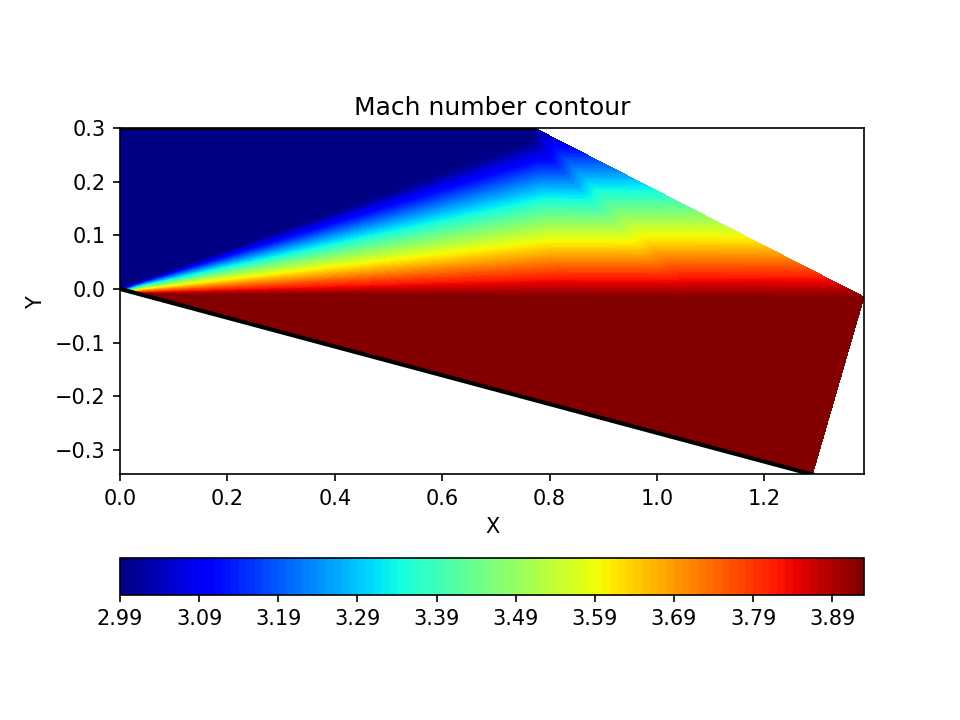
\includegraphics[scale=0.9]{results/expansion_corner/M_contour.png}
    \caption{Mach number contour output from computation}
    \label{Mach_contour}
\end{figure}

\begin{figure}
    \center
    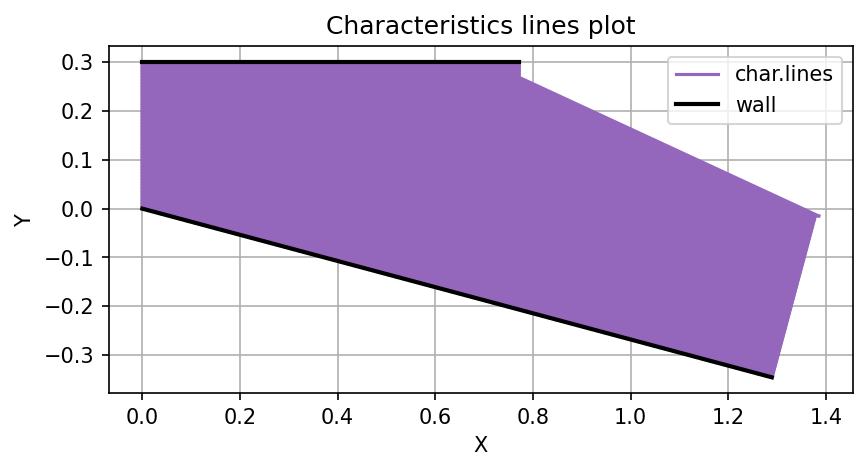
\includegraphics[scale=0.9]{results/expansion_corner/char_map.png}
    \caption{characteristic points distribution (conjested due to 18k points for N = 100)}
    \label{char_output}
\end{figure}

\par Further, the Mach number of downstream section after expansion, obtained
from the computation is compared with the theoretical value obtained
from \cite{ref_1}. The following gives the values obtained and they found to
be in agreement with the theory.
\begin{align*}
    M_{2,computation} &= 3.92329 \\
    M_{2,theory} &= 3.923
\end{align*}

\pagebreak


\begin{thebibliography}{2}
    \bibitem{ref_1} Online Prandtl-Meyer expansion flow calculator; https://www.omnicalculator.com/physics/prandtl-meyer-expansion
    \bibitem{ref_2} Michel A. Saad; Compressible fluid flow

\end{thebibliography}

\pagebreak

\begin{appendices}
    \section{Appendix - Python code of Question 1}\label{appendixA}
    This section contains the \emph{Python} code developed for the MOC computation

    \lstinputlisting[language=Python]{results/expansion_corner/script_expansionCorner_MOC.py}

\end{appendices}

\par
\center{**********}

\end{document}
